\section{Back Propagation}
Now a Neural Network could be programmed with all showed on \ref{sec:hood}, a program that output $y_1,$ and $y_2$ could be developed. But, where is the "learning" of deep learning here? Nowhere, yet. Is the moment of teaching the net with examples, giving it some inputs and showing it the expected outputs. The \textit{Back Propagation Algorithm} is going to achieve it. The goal of this method is to minimize the error using the method of gradient descent.

\subsection{Activation Function}
As explained before each neuron has to apply one function to the result of its computing. One of the most popular functions used for this purpose is the sigmoid:
\begin{equation}
  s(x)=\frac{1}{1+e^{-cx}}
\end{equation}
The shape of this function depends on the value of $c$, but for simplicity $c=1$ is going to be used. The derivate of the sigmoid function respect of x is $s(x)^\prime=s(x)(1-s(x))$. One of the reasons why this function is used is the simplicity of the derivate, because it allows to make all the derivates later more easily ~\cite[Chapter~7]{rojas}.
\begin{figure}
  \center
  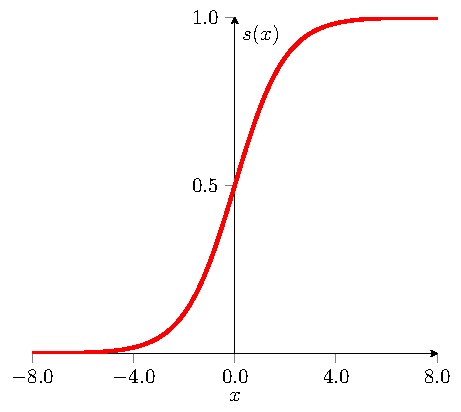
\includegraphics{images/sigmoid.pdf}
  \caption{Shape of the sigmoid with $c=1$}
\end{figure}

\subsection{The Error}
The error could be measured in differents ways. The most common and apparently most effective method is to calculate the Euclidean distance. It allows to measure the error in different dimensions, for example, the error in $\rm I\!R^1$ between $4$ and $1$ is $E=4-3=1$. For $\rm I\!R^2$ you should use the Pythagorean theorem, and for $\rm I\!R^n$ the distance is:
\begin{equation}
  E_{(p,q)}=\sqrt{(p_1-q_1)^2+(p_2-q_2)^2+\dots+(p_i-q_i)^2+\dots+(p_n-q_n)^2}
\end{equation}

Is important to know how to size the error that the net has because you have to tell the network how far was the result from the expected output. And only once you have the distance between the target and the output you can adjust the knobs to achieve a better result.

How much the knob must be changed? It depends on how important is that knob for the result. For example it might be possible that changing one knob will get the same result. In this case it does not matter if we adjust the knob, but, what about one knob that when adjusted change the result drastically? Here the new position of the knob is realy important. Hence we need the partial error with respect a specific weight or bias ~\cite[Chapter~2]{nielsen}:
\begin{equation}
  \frac{\partial e}{\partial w^{(k)}_{ij}} \quad \textrm{or} \quad \frac{\partial e}{\partial u^{(k)}_{i}}
\end{equation}

\subsection{The Correction}
Once we can calculate the error depending on one parameter we are ready to make the correction to the network. The process is simple, first you feed the input layer with some data, then you get the result and compare it with the target and finally you make this adjustment for each weight and bias (the $\alpha$ is the learning constant and represent how far is the next step in the gradient descent) ~\cite[Chapter~7]{rojas}:
\begin{equation}
\begin{aligned}
  w^{(k)}_{ij} & \Rightarrow & w^{(k)}_{ij} - \alpha \frac{\partial e}{\partial w^{(k)}_{ij}} \\
  u^{(k)}_{i} &  \Rightarrow & u^{(k)}_{i} - \alpha \frac{\partial e}{\partial u^{(k)}_{i}}
\end{aligned}
\label{eq:corr}
\end{equation}

To develop a working neural network is now possible with all this knwoledge. First we have to declare the architecture of our net. Then we set random weights and biases and we start teaching the net. Imagine you have a 10.000 images dataset, then you take 90\% of those images to train the net, and the other 10\% for testing how well we have developed it. We feed the network with one of those images from the train set and make the correction as we have seen in \ref{eq:corr}. Ideally we should do it with all the train set but as the size of that set could be (and should be) huge, we just take a small batch representative and apply the correction for each image of the batch. Once we have done it we have complete one epoch. With just one epoch the network still giving us weird answers, so what we have to do is to train the network with several epochs and then our network is trained and ready.

To measure how intelligent our network is you can use the test set of images to calculate the accuracy.
